\chapter{Computational Frameworks}

\section{Background}
\quad For many decades there has been an ongoing trend in the process of software engineering to move up in the levels of abstraction from a bare hardware to a higher level concepts closer to a human reasoning and understanding. There have been several breaking points. A move from assembly languages to languages like Fortran and C increased the productivity of programmers by supporting structuredness and modularity and offloading many routine and tedious tasks onto a compilation software. C and Fortran were high-level languages of that time, but still a low-level languages for today's standards. These languages support an imperative programming paradigm. The main characteristic of that is the concept of state. The statements of the language read and update the state. Procedures pass the state and results around achieving the final goal of the program.   

\quad The trend of moving from low to higher abstraction levels is not only true for software engineering in general, but for parallel software engineering in particular. Modern hardware provides a diverse and vast support for different forms of parallelism: pipelined CPUs with out-of-order and superscalar instruction execution, vector extensions of modern CPU instruction sets, multi-core processors running as part of multi-processor system, etc. Given a sequential program a programmer can work at the finest level of granularity by choosing vector instructions over scalar ones and changing their relative order trying to minimise the number of pipeline stalls and memory waits. To exploit a coarse-grain parallelism a programmer can rewrite a program in a multi-threaded fashion. Here a programmer may choose to work with the operating system interface like POSIX threads or use some 

abstract parallel machine models   


level by rewriting program instructions by preferring vector ones to a scalar or change their relative order trying to minimise the number of pipeline stalls    

in modern computing systems a programmer may 

sequential program a programmer can work with its instructions directly by 



\subsection{Automatic Data Structure Recognition}

\subsection{OOP and Software Design Patterns}
\quad Object-oriented software design is a complex topic in itself, which spawns a number of problems and questions. 

\quad Software design patterns are reusable solutions to common design problems in object-oriented software engineering. They live at the level higher than that of a source code and are language agnostic. The solutions can be regarded as standard solutions to design problems they target. These solutions have been well tested and proven to be the most reliable and elegant.

Chain of responsibility pattern is very similar to fold.
Visitor pattern roughly corresponds to fold.

\subsection{Imperative and Functional programming}
\quad Programming languages can be classified by different programming paradigms they support. Among the most general classifications are imperative and declarative programming paradigms.\newline\null
\quad Imperative programs are written in a form of instruction sequences, which read and write the state of a program. The concept of state is the main characteristic of imperative programming paradigm. Instruction sequences can be structured in various ways. In procedural programming paradigm instructions are grouped inside procedures and functions. In object-oriented programming (OOP) paradigm instructions are grouped with the data they operate on inside objects of various types or classes.\newline\null
\quad Declarative programs do not specify the exact sequence of steps and state updates a program needs to do in order to get the desired result. Declarative programs declare the properties of the desired result. The properties can be specified as a set of constraints like in constraint programming or a set of linear inequalities like in linear programming. Functional programming is another subtype of declarative programming. In functional programming the final desired result is specified as a sequence of stateless function evaluations. Among the most common functions are map, reduce, fold, etc.

\subsection{Parallel Algorithmic Skeletons}




\section{Computational Frameworks}
\quad In this work we propose an idea of \textbf{computational frameworks} and we show its utility and use on a subset of Olden benchmarks. The idea grows on a wide review of the available parallel software development methodologies as well as on the understanding of problems in the task of software parallelization.  

\subsection{Overview}
\quad In our project we propose a C++ library of computational frameworks. Computational frameworks are a blend of imperative, object-oriented and functional programming paradigms. They lift algorithm implementation in the C++ language to a higher level.
Computational frameworks are a blend of algorithms and data structures as well as several programming paradigms such as imperative, object-oriented and functional programming. They lift C++ program implementations to a higher conceptual level. 

User-exposed methods of classes are higher-order functions and can take custom function objects, function pointers, lambda functions and apply them to framework elements in a framework defined way. Unlike pure functions the application of user-defined functions to our computational frameworks can have side-effects.

\quad Improves structuredness, modularity, separation of concerns and hides possible program parallelization behind the convenient user API.  

\subsection{Fractal}
\quad The \textbf{Fractal} computational framework has been inspired by the theoretical work on tree reductions [] and 3 Olden benchmarks (health, treeadd, perimeter). Figure \ref{fig:fractal} illustrates the Fractal functionality.\newline\null
\quad There are numerous data structures, computational patterns, processes and examples, which can be characterized as being fractals.\newline\null
\quad The simplest example of fractal is an n-ary tree. Imagine we store some data at every node of the tree and want to accumulate it starting from the leaves at the very bottom and going all the way up to the root of the tree. Accumulation procedure processes every node by taking the result from all its children, making a computation and passing the result up to the parent element. The procedure may have some side-effects on the nodes and keeps the whole tree data structure along with its state in memory. In that sense it is not a stateless functional programming. At the same time the accumulation procedure can be passed as an argument to a higher-order compute function. The movement of data through the nodes of the tree from their children to their parents is the fixed and immutable part of an algorithm, whereas the accumulation procedure can be given as a parameter. The latter separates the algorithm into a well-structured user and library parts. The library part acts as a backbone and the user part grows on it. The computations described above lie at the basis of health and treeadd benchmarks.\newline\null
\begin{figure}[ht]
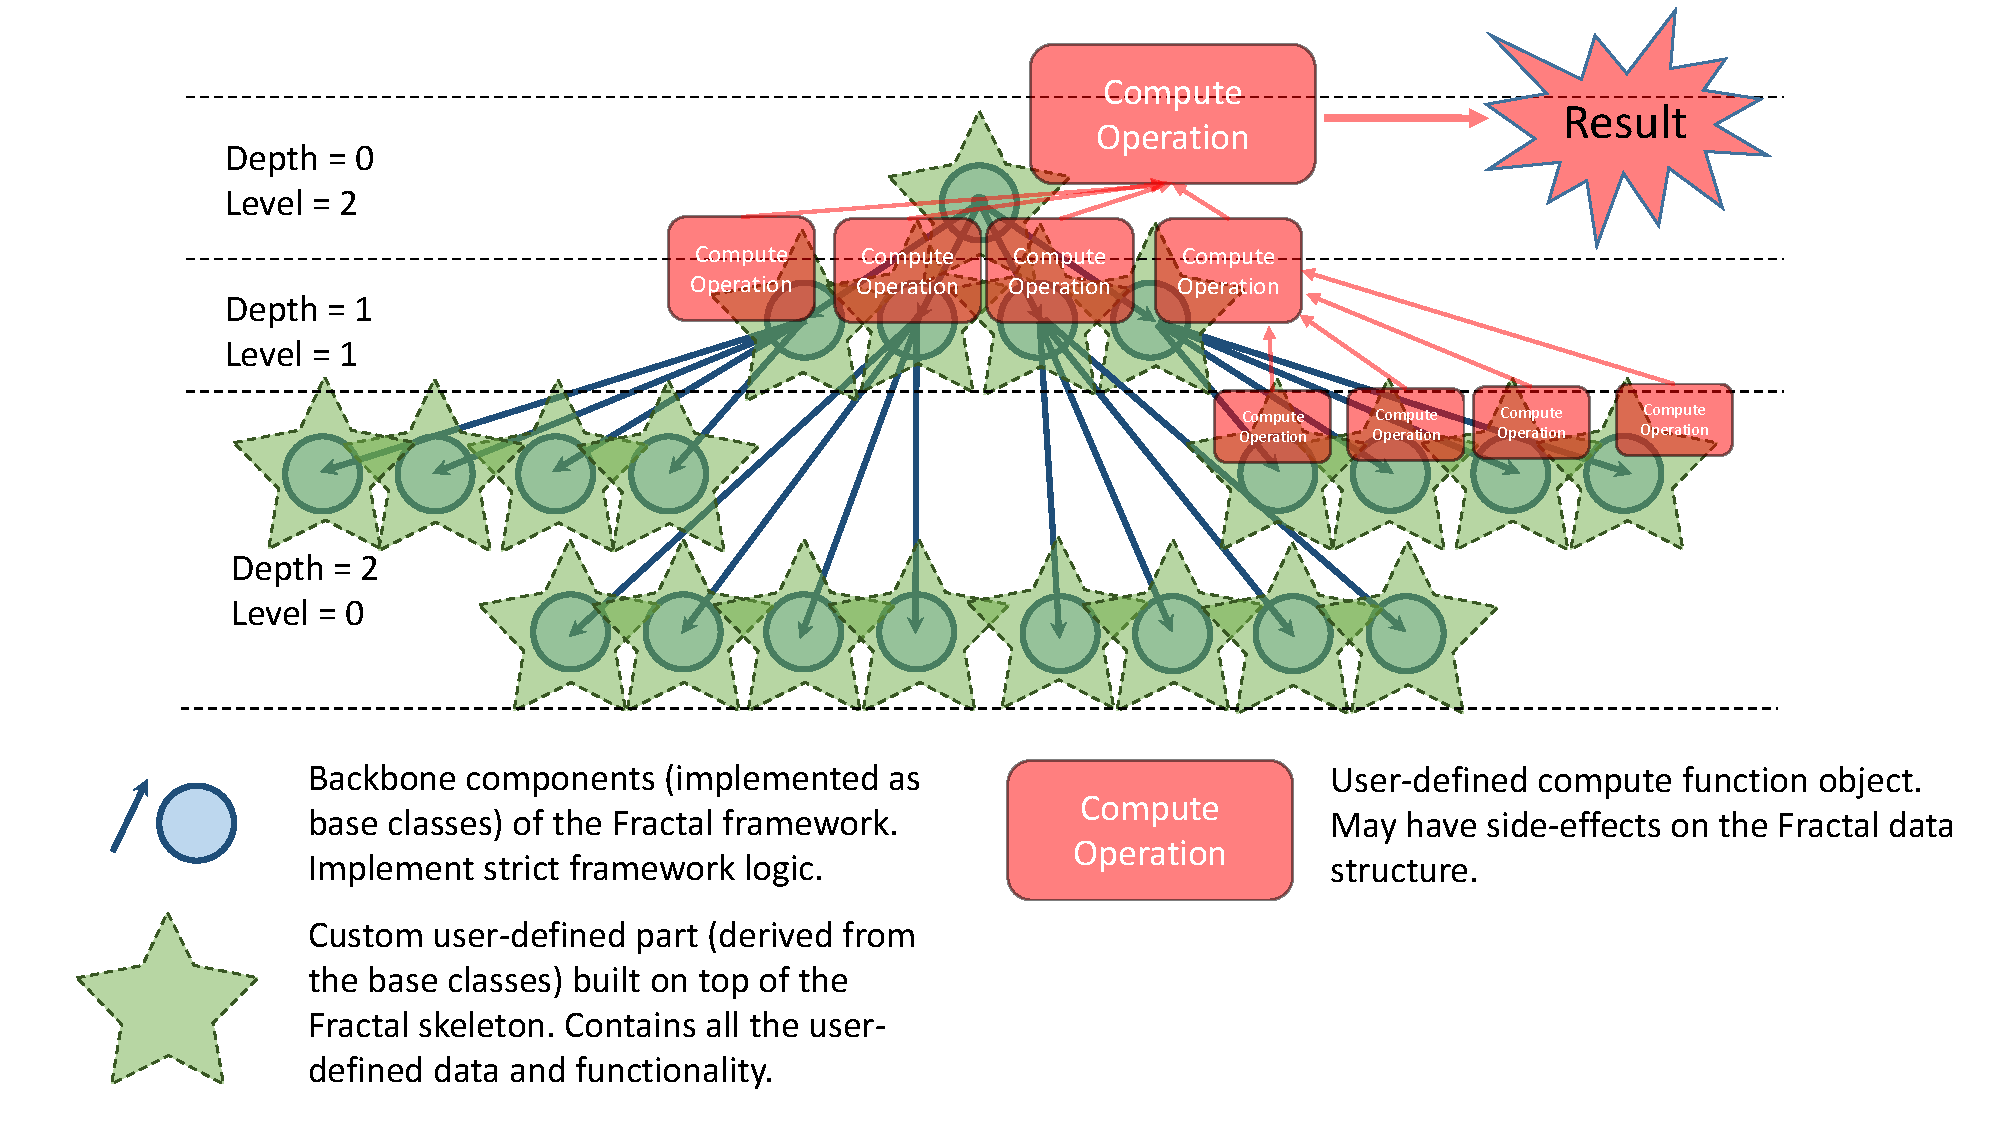
\includegraphics[width=1.0\textwidth]{images/Fractal.pdf}
\caption{The Fractal computational framework.}
\label{fig:fractal}
\end{figure}
\quad A more complicated and interesting fractal example would be a square being continuously and recursively divided into 4 equal sub-squares (southwest, northwest, southeast and northeast). The deep-growing structure is actually a 4-ary tree as well. Imagine one wants to compute the perimeter of some figure. One way to do it would be to map the figure on the square plane and then turn the plane into a grid by continuously splitting the square into 4 equal sub-parts (southwest, northwest, southeast, northeast) till we reach the granularity size of the grid. Then we paint all the grid elements located inside the figure shape as black and those outside of it as white. We iterate over the grid and detect all points of color flips and add the size of the grid elements to the final sum, which at the end is going to approximate the perimeter of the figure. That is roughly what the perimeter benchmark does.\newline\null
\quad In all its generality the fractal is a pattern, which can be characterized with self-similarity, repeatedness, structuredness, inherent parallelizability and the exact numeric values such as its depth and arity. All that naturally maps onto the C++ implementation as a class template we describe below.
\subsection{Fold}

\subsection{Reduce}



\subsection{Frameworks Library Design}
\quad The computational frameworks are designed as a set of C++ class templates. The user interface these templates provide has been designed and refined iteratively using the set of Olden benchmarks [].     

\begin{minipage}[t]{\linewidth}
\begin{lstlisting}[caption={Computational framework class template skeleton},label={lst:framework_template_skeleton},language=C++]

template <typename ElemType, typename SeedType>
class Framework {
    public:
        class Element {
            // user-exposed customization iface
            virtual void grow(SeedType) = 0;
            virtual bool growth_stop_condition() { return false; }
        };
        template <typename ComputeType>
        class ComputeFunction {
            // framework specific application function API
            virtual operator()(ElemType& elem, ... ) = 0;
            virtual operator(const std::vector<ComputeType>&) = 0;
*       };
   /     
        void grow(size_t size, SeedType seed) {
            // organise framework elements 
            // into a data structure
            ... = new ElemType(); 
        }
        template<typename ComputeType>
        ComputeType compute(ComputeFunction<ComputeType>& apply_func);
    
    private:
        // framework data structure organisation
        // (list, tree, array, etc.)
};

\end{lstlisting}
\end{minipage}

\quad The design and the implementation of our template library reflect the target goals of the concept of computational frameworks.    

\quad There were several questions raised in the design process of a template library. 




\subsection{Fractal}
\quad The fractal computational framework



\subsection{Fold}
\quad Fold abstracts away common patterns of recursion.


\subsection{Reduce}

